\slide{firewalls}

\begin{list1}
\item Indeholder typisk:
  \begin{list2}
   \item Grafisk brugergr�nseflade til konfiguration - er det en
   fordel?
\item TCP/IP filtermuligheder - pakkernes afsender, modtager, retning
  ind/ud, porte, protokol, ...
\item kun IPv4 for de kommercielle firewalls
\item b�de IPv4 og IPv6 for Open Source firewalls: IPF, OpenBSD PF,
  Linux firewalls, ...
\item foruddefinerede regler/eksempler - er det godt hvis det er nemt
  at tilf�je/�bne en usikker protokol?
\item typisk NAT funktionalitet indbygget
\item typisk mulighed for nogle serverfunktioner: kan agere
  DHCP-server, DNS caching server og lignende
  \end{list2}
\item En router med Access Control Lists - kaldes ofte netv�rksfilter,
  mens en dedikeret maskine kaldes firewall
%  funktionen er reelt den samme - der filtreres traffik
\end{list1}

\slide{regels�t fra OpenBSD PF}

\begin{list1}
\item \begin{alltt}
\tiny 
# hosts
router="217.157.20.129"
webserver="217.157.20.131"
# Networks
homenet="{ 192.168.1.0/24, 1.2.3.4/24 }"
wlan="10.0.42.0/24"
wireless=wi0

# things not used
spoofed="{ 127.0.0.0/8, 172.16.0.0/12, 10.0.0.0/16, 255.255.255.255/32 }"

block in all # default block anything
# loopback and other interface rules
pass out quick on lo0 all
pass in quick on lo0 all

# egress and ingress filtering - disallow spoofing, and drop spoofed
block in quick from $spoofed to any
block out quick from any to $spoofed

pass in on $wireless proto tcp from $wlan to any port = 22
pass in on $wireless proto tcp from $homenet to any port = 22
pass in on $wireless proto tcp from any to $webserver port = 80

pass out quick proto tcp  from $homenet to any flags S/S keep state
pass out quick proto udp  from $homenet to any         keep state
pass out quick proto icmp from $homenet to any         keep state
\end{alltt}
%$
\end{list1}

\slide{netdesign - med firewalls}

\begin{center}
\colorbox{white}{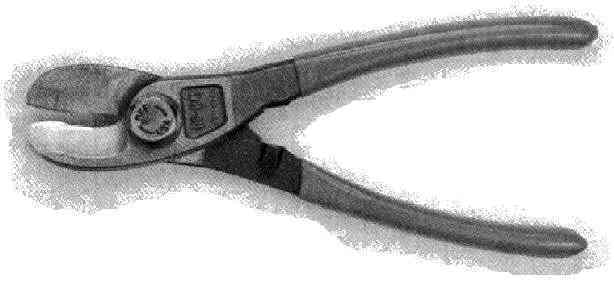
\includegraphics[width=12cm]{images/kut.jpg}}  
\end{center}

\begin{list2}
\item Hvor skal en firewall placeres for at g�re st�rst nytte?
\item Hvad er foruds�tningen for at en firewall virker?\\
At der er konfigureret et s�t fornuftige regler!
\item Hvor kommer reglerne fra? Sikkerhedspolitikken!
\item Kan man lave en 100\% sikker firewall? Ja selvf�lgelig, se!
\end{list2}


{\small Kilde: \link{http://www.ranum.com/pubs/a1fwall/} The ULTIMATELY Secure Firewall}
%\href
%{http://www.ranum.com/security/computer\_security/papers/a1-firewall/}
%{http://www.ranum.com/security/computer_security/papers/a1-firewall/}
% old link: 


%%% Local Variables: 
%%% mode: latex
%%% TeX-master: t
%%% End: 
